\documentclass[]{article}
\usepackage[english,german]{babel}
\usepackage{cite}
\usepackage{graphicx}
\usepackage{tabularx}
\usepackage{subcaption}
\usepackage[utf8]{inputenc}
\captionsetup[subfigure]{list=true, font=large, labelfont=bf, 
	labelformat=brace, position=top}


%opening
\title{Überblick über die elektronischen Systeme von Fahrzeugen}
\author{
	Peter Burger
	\and
	Malte Hoffmann
	\and
	Andreas Lay
	\and
	Benjamin Pottkamp
	\and
	Tobias Schlauch
	\and
	Tobias Wiest
}
\date{14. Februar 2020}

\begin{document}
\sloppy

\maketitle

\begin{abstract}
	Mittlerweile machen elektronische Systeme etwa ein Drittel der Gesamtkosten bei der Produktion von
	Personenkraftwagen aus \cite{BP01} Von Motorsteuerung, über aktive und passive Sicherheitssysteme, 
	Wartung und Diagnose bis hin zur Unterhaltungselektronik sind Personenkraftwagen inzwischen hochgradig
	vernetzte Systeme.\\
	
	Mit den aktuellen Entwicklungen in Richtung teil- und vollautonomer Systeme wird diese Vernetzung noch weiter zunehmen 
	und die elektronischen Systeme werden in absehbarer Zukunft Hauptwertträger eines Fahrzeugs werden.\\
	
	Ziel dieser Ausarbeitung ist es dem interessierten Leser einen Überblick über die wichtigsten elektronischen Systeme in
	modernen Fahrzeugen und deren Interaktion untereinander zu geben. Ein gewisses technisches Grundverständnis vorrausgesetzt 
	soll er in der Lage sein, neue Entwicklungen in den Kontext des aktuellen Stand der Technik zu setzen.\\
	
	Da es sich um ein komplexes Thema handelt, dass auf beschränktem Platz dargeboten werden soll, müssen gewisse Teilbereiche naturgemäß
	kürzer ausfallen oder gänzlich ignoriert werden, weshalb diese Arbeit als Ausgangspunkt für eine nähere Beschäftigung mit dem Thema
	zu verstehen ist.
\end{abstract}

\tableofcontents

%including the separate Files
%\section{Vernetzung}
Mit neuen Anforderungen an die Sicherheit und Effizienz, sowie einer Vielzahl von gewünschten Features 
für Komfort und Unterhaltung, zeichnet sich ein enormer Anstieg der in modernen Fahrzeugen verbauten ECUs ab \cite{TW_kim2014gateway}.
Ein Großteil dieser Systeme und Steuergeräte ist voneinander abhängig. Zentral erfasste Signale werden von mehr als nur einem
System benötigt und verarbeitete Signale, sowie berechnete Werte müssen zwischen zusammenhängenden Systemen vermittelt werden.

Mit einer herkömmlichen Verkabelung der einzelnen Komponenten wie zum Beginn der Automobilindustrie ist ein derartiges Wachstum
nicht zu bewältigen \cite{leen1999digital}. Neben Problemen wie erhöhtes Gewicht und Kosten einer solchen Verkabelung bietet ein solches System keine
Composability \cite{reif2011bosch}. Dies hat zur Folge dass neue Teilkomponenten nicht in das Gesamtsystem integriert werden können, ohne die Funktion 
weiterer Teilkomponenten zu beeinflussen. Somit ist eine modulare Zusammensetzbarkeit des internen Kommunikationsnetzwerkes eines Fahrzeugs nötig, um die 
steigende Komplexität der verbauten Elektronik zu bewältigen \cite{reif2011bosch}.

Im Hinblick auf die erhöhte Komplexität der Elektronik und die daraus folgenden Anforderungen werden wir im Folgenden
einen Überblick über die Topologie, Technologien und Netzwerkprotokolle, sowie die Unterteilung und Kopplung des internen Netzwerks eines Fahrzeugs bieten.

    \subsection{Topologie}
    Die Topologie des Netzwerkes spiegelt die Anordnung der Knoten und Leitungen des Netzwerks wieder. Sie bildet ab in welcher Weise Daten zwischen
    den einzelnen Knoten ausgetauscht werden können. Je nach Anforderungen an das Netzwerk werden unterschiedliche Topologien verwendet,
    welche einen weitreichenden Einfluss auf die Eigenschaften des Teilnetzwerks als auch des Gesamtsystems haben.
        \begin{itemize}
            \item Ringtopologie: Hier sind die Netzwerkknoten in einem Ringschluss verbunden. Der Zugriff auf das Medium erfolgt typischerweise sequentiell 
            oder mittels eines Tokens. Es gibt sowohl unidirectionale als auch bidirectionale Ringstrukturen. Bei letzterem existiert ein gegenläufiger Ring, 
            sodass beim Ausfall einer Station nicht das gesamte Netzwerk betroffen ist. FDDI etwa ist ein derartiger Dual-Ring.
            \item Sterntopologie: Bei dieser Topologie sind die einzelnen Knoten mit einem zentralen Knoten verbunden. Der Ausfall eines Links beeinflusst lediglich
            eine Station aber durch den zentralen Knoten existiert ein Single-Point-Of-Failure. 
            \item Maschentopologie: Hierbei werden die Knoten des Netzwerks direkt miteinander verbunden, in einem vollvermaschten Netz besitzt jeder Knoten eine 
            dedizierte Verbindung zu allen anderen Knoten im Netzwerk. Vorteile sind hohe Ausfallsicherheit und schnelle Datenübertragung. Jedoch steigt die Anzahl der 
            nötigen Verbindungen in einem vollvermaschten Netzwerk quadratisch an.
            \item Bustopologie: Bei dieser Topologie sind alle Knoten mit einem einzigen Übertragungsmedium verbunden. Fällt eine Station aus, so ist der Rest des Netzwerks
            nicht betroffen. Da mehrerer Stationen auf das selbe Medium zugreifen kommen entsprechende Zugriffsverfahren zum Einsatz. Vorteile sind etwa gerine Kosten und die
            einfache Erweiterung um neue Knoten.
            \item Hybridtopologie: Oftmals sind auch hybride Varianten der genannten Topologien anzutreffen. Beispielhaft ist eine Stern-Ring-Topologie denkbar, indem
            mehrere Ringe über einen zentralen Hub oder Switch verbunden werden.
        \end{itemize}
    \subsection{Zugriffsverfahren}
    Für unterschiedlich verwendete Technologien und Anforderungen können verschiedene Zugriffsverfahren genutzt werden. Diese sind nötig um Kollisionen bei gleichzeitigem,
    schreibenden Zugriff durch mehrere Knoten eines Netzwerks auf das selbe Übertragungsmedium zu verhindern. Im Folgenden werden einige Möglichkeiten kurz dargestellt.
        \begin{itemize}
            \item TDMA: Time Division Multiple Access ist ein Verfahren bei dem die Zugiffszeit in Zeitslots unterteilt wird, welche den entsprechenden
            Stationen des Netzwerks zugeordnet werden. Dadurch können Kollisionen vermieden werden, da Knoten nur in den ihnen zugeteilten Zeitslots Signale 
            senden. Bei geringer Auslastung ist ein derartiges Verfahren jedoch suboptimal, da die Gesamtzugriffszeit nicht effektiv ausgenutzt werden kann.
            \item FDMA: Frequency Division Multiple Access ist ein Multiplexingverfahren bei dem die verfügbare Bandbreite in nicht-überlappende Frequenzbereiche aufgeteilt wird,
            um das Senden von Daten durch mehrere Knoten zum selben Zeitpunkt zu ermöglichen.
            \item CDMA: Code Division Multiple Access ist eine Form von Multiplexing, welche es erlaubt das mehrere Teilnehmer gleichzeitig im selben Frequenzbereich
            senden können. Hierfür werden Spreizcodes verwendet, welche ermöglichen dass mehrere Stationen zur selben Zeit unterschiedlich codierte Daten senden können.
            Anhand dieser Codierung können die Datenströme bei Empfängern wieder getrennt werden.
            \item Token Passing: Hierbei handelt es sich um ein Zugriffsverfahren welches etwa bei Token-Ring oder FDDI zum Einsatz kommt. Die Sendeerlaubnis ist bei diesem
            Verfahren abhängig vom Besitz eines authoritativen Tokens, welches innerhalb des Netzwerks weitergereicht wird.
            \item CSMA/CD: Carrier Sense Multiple Access / Collision Detection ist ein Zugriffsverfahren welches bei Ethernet Anwendung fand. Dabei lauschen teilnehmende Stationen
            auf dem gemeinsam genutzten Medium auf Übertragungen. Ist das Medium frei, können Daten gesendet werden. Hierbei lassen sich Kollisionen jedoch nicht vermeiden, sondern lediglich 
            erkennen. 
            
            Sobald während des eigenen Sendevorgangs weitere Signale ausgehend von einer anderen Quelle erkannt werden, wird die Übertragung abgebrochen. Anschließend wird ein
            Jam-Signal ausgesendet und eine gewisse Zeitspanne gewartet bevor der Prozess erneut beginnt (Lauschen auf Belegung des Mediums, Sendeversuch und Kollisionserkennung).
            Aufgrund der Etablierung von Switched Ethernet und der entstehenden kollisionsfreien Domänen wird CSMA/CD kaum noch benötigt. Im WLAN wird CSMA/CA verwendet.
        \end{itemize}
    \subsection{Kommunikation}
    Die eigentliche Datenkommunikation in einem Netzwerk kann anhand der Adressierungsart, sowie verwendeten Steuermechanismen unterschieden werden. 
    
    So ist die am häufigsten vorzufindende Adressierungsart teilnehmerorientert. Grundlage dieser Form des Datenaustauschs sind Knotenadressen, welche zusammen mit den
    zu übertragenden Daten die eigentliche Nachricht bilden \cite{reif2011bosch}. Diese Form der Adressierung finden wir etwa bei Ethernet oder IP. 
    
    Eine weitere Adressierungsart welche im Kontext des Automobils von Relevanz ist, ist die nachrichtenorientierte Adressierung. Hierbei werden nicht Empfänger, sondern die Nachrichten selbst
    adressiert, indem sich ein Identifier in den Nachrichten befindet, welcher den Nachrichtentyp kennzeichnet \cite{reif2011bosch}. In diesem Fall benötigt der Sender keine 
    Kenntnisse über Teilnehmer bzw. deren Adressen und jeder Empfängerknoten entscheidet selbstständig ob er eine Nachricht verarbeitet \cite{reif2011bosch}. Später betrachtete
    Protokolle wie CAN, LIN und Flexray sind nachrichtenorientierte Protokolle.

    Auch Anhand der Steuermechanismen kann die Kommunikation in Netzwerken unterschieden werden. Unterschieden wird zwischen ereignis- und zeitgesteuerten Systemen.
    Ereignisgesteuerte Bussysteme können aufgrund der inhärent fehlenden Synchronisation der Nachrichten und folglich entstehenden Kollisionen beim Zugriff auf den Bus
    überlastet werden, sollte die Anzahl der interagierenden Knoten zu hoch sein \cite{reif2011bosch}. Besonders gut geeignet sind derartige Systeme für unerwartete Ereignisse,
    welche idealerweise ohne Latenz im Vergleich zu zeitgesteuerten Systemen übertragen werden können \cite{reif2011bosch}. Beispielhaft hierfür sind jegliche Interaktionen eines 
    Fahrzeugführers mit dem System. Bei erhöhten Anforderungen bezüglich der Sicherheit und Zuverlässigkeit eines Systems bieten sich wiederum zeitgesteuerte Systeme an \cite{reif2011bosch}.
    Elektronische Brems- und Lenksysteme benötigen derartige zeitliche Zusicherungen.
    \subsection{Technologie}
    Nachdem wir einige grundsätzliche Aspekte und Terminologien bezüglich der Vernetzung und Kommunikation betrachtet haben, geben wir im folgenden einen kurzen Überblick
    über verwendete Technologien und Netzwerkprotkolle, welche wir je nach Relevanz in einer späteren Sektion noch einmal aufgreifen und genauer betrachten werden.
        \subsubsection{Wired}
        Im folgenden gegen wir einen Überblick über die am meisten verbreitetsten Netzwerkprotokolle in heutigen Fahrzeugen. 
            \begin{itemize}
                \item CAN (Controller Area Network): CAN wird seit langer Zeit für den Großteil der Datenkommunikation in Fahrzeugen verwendet \cite{leen1999digital}.
                Vorallem im Bereich des Antriebsstrangs, Fahrwerks sowie den Systemen zur Kontrolle des Innenraums ist CAN als bevorzugte Netzwerktechnologie vorzufinden.
                CAN ist ein asynchroner serieller Bus Standard, welcher Steuergeräte, Sensoren und Aktoren zu einem System verbindet. 
                
                Es handelt sich um ein Multi-Master-Kommunikationsprotokoll welches für Datenintegrität und Automobilapplikationen mit Datenraten von 1 MB/s geschaffen wurde \cite{wolf2004security}. Vorteile
                dieser Technologie sind die geringen Kosten und hohe Zuverlässigkeit. Eingeschränkt ist die Technologie durch die geringe Bandbreite, weshalb Sie
                ungeeignet für Unterhaltung und Medienstreams ist \cite{TW_huang2018vehicle}.
                \item LIN (Local Interconnect Network): LIN ist ein asynchrones, single-master, multi-slave Netzwerkprotokoll, welches in Hinblick auf Kostenersparnis 
                designed wurde. Eingesetzt wird LIN vorallem für Low-Speed-Kommunikation und stellt eine kosteneffiziente Alternative dar um Motor und Sensoren innerhalb 
                eines Fahrzeugs zu verbinden. Typischerweise kommt es bei der Elektronik des Innenraums, wenn die Bandbreite von CAN nicht benötigt wird, wie z.B bei Türheber
                oder der Sitzanpassung zum Einsatz \cite{TW_huang2018vehicle}.
                \item Flexray: Flexray wurde als eine schnellere, zuverlässige aber auch teurere Alternative zu CAN entwickelt. Es handelt sich um ein Kommunikationsprotokoll mit einer
                Dual-Channel Datenrate von bis zu 10 MB/s für komplexere Kontrollsysteme innerhalb eines Fahrzeugs \cite{wolf2004security}. Über die Dual-Channel Architektur kann die Zuverlässigkeit
                bei Anwendungen wie Brake-By-Wire gewährleistet werden \cite{TW_huang2018vehicle}. 
                \item MOST (Media Oriented Systems Transport): MOST ist eine High-Speed Netzwerk Spezifikation welche speziell für Übertragung von Medien wie Audio und Videosignalen 
                geschaffen wurden. Es handelt sich dabei um einen seriellen Bus welcher eine Ringtopologie verwendet \cite{TW_huang2018vehicle}.
                \item Ethernet: Als Standardtechnologie für drahtgebundene lokale Netzwerke spielt Ethernet eine kritische Rolle bei jeglicher Art von Kommunikation.
                Vorteile von Ethernet als Mittel zur Vernetzung gegenüber bereits genannten Technologien ist die deutlich höhere Bandbreite, Skalierbarkeit und Flexibilität \cite{hank2013automotive}\cite{TW_huang2018vehicle}. 
            \end{itemize}
        \subsubsection{Wireless}
        Als alternatives Mittel zur herkömlichen verdrahteten Kommunikation zwischen den Komponenten eines Fahrzeugs existieren auch einige drahtlose Technologien.
        Diese können nicht nur zur Verbindung zwischen persönlichen Geräten des Fahrers mit dem Fahrzeug, sondern auch zur Verbindung der internen Systeme genutzt werden.
        Damit könnte ein Großteil der Sensoren, Aktoren und ECUs drahtlos verbunden werden.
            \begin{itemize}
                \item WLAN: Der Standard IEEE 802.11 wurde als drahtlose Alternative zu kabelgebunden High-Speed
                Netzwerken geschaffen. Auch im Automobil kann WLAN genutzt werden um persönliche Geräte wie Smart Phones,
                Tablets und Laptop mit dem Unterhaltungssystem des Fahrzeugs zu verbinden \cite{TW_huang2018vehicle}. 
                \item Bluetooth: Bluetooth wurde für drahtlose Kurzstrecken-Kommunikation designed. Optimiert wurde die
                Technologie für Audiostreams und ist idealerweise für drahtlose Lautsprecher eines mobilen Audiosystems geeignet.
                Auch händefreies Telefonieren über eine Verbindung zum Smart-Phone ist bereits im Großteil der modernen Fahrzeuge 
                über Bluetooth möglich.
                
                BLE (Bluetooth Low Energy 4.0) ermöglicht Verbindungen mit geringer Latenz, hoher Zuverlässigkeit
                und geringem Energieverbrauch, weshalb der Einsatz dieser Technologie zur Verbindung von Sensornetzwerken und ECUs im Innenraum, 
                dem Antriebsstrang und Fahrwerk denkbar wären \cite{TW_huang2018vehicle}. Für kritische Systeme wie Brems- und Lenksysteme bleibt der Einsatz jedoch bedenklich \cite{wolf2004security}.
                \item UWB (Ultra-Wideband): UWB ist eine Radiowellen Technologie für kurze Entfernung und hohe Bandbreite, welche als Alternative zu Wifi und Bluetooth gesehen werden kann.
                \item Zigbee: Zigbee ist ein kabelloser Standard, welcher auf dem Standard 802.15.4 beruht und Geräte mit geringerem Datendurchsatz und niedrigem Energieverbauch in einem 
                Mesh-Netzwerk verknüpft. Die Datenraten reichen bis zu 250 KB/s. Zigbee kann genutzt werden um ECUs, Sensoren und Aktoren in einem Fahrzeug zu verbinden \cite{TW_huang2018vehicle}.
            \end{itemize}
    \subsection{Systemunterteilung}
    Mit dem Einzug einer Vielzahl neuer Systeme für die Unterhaltung, Navigation, On-Board Diagnostik,
    Augmented Reality (AR) Dashboards oder etwa Fahrassistenzsysteme finden wir in aktuellen Top-Modellen bereits 
    ca. 70 ECUs \cite{TW_huang2018vehicle}. Mit steigender Anzahl und zunehmender Komplexität 
    benötigen diese ECUs eine größere Bandbreite und geringere Latenz des internen Netzwerks \cite{TW_huang2018vehicle}.
    Das Gesamtsystem lässt sich hierbei in die 4 Bereiche Powertrain, Chassis, Innenraum und Telematik unterteilen.
        \subsubsection{Powertrain}
        Der Antriebsstrang umfasst alle Komponenten welche für die Leistungserzeugung für den Antrieb verantwortlich sind. Dies umfasst 
        den Motor, Getriebe, Antriebswelle, Räder etc. Von Relevanz sind hierbei etwa die Engine Control Unit oder das Powertrain Control Module.
        Auch Sensoren und Aktoren, etwa zur Erhebung und Regulation von Geschwindigkeit, Drehzahl, Öl-Stand, Zylinderdruck, Position, Stabilität sind hierbei miteinbegriffen \cite{IVN}.
        Im Bereich des Antriebstrangs stehen Echtzeitanwendungen im Vordergrund \cite{reif2011bosch}\cite{TW_huang2018vehicle}.
        \subsubsection{Chassis}
        Das Fahrwerk umfasst alle Komponenten welche den Antriebsstrang und die Karosserie tragen. Bekannte Komponenten sind etwa
        Bremsen, Lenkung und Federung. Hier finden wir eine Vielzahl von Sensoren und Aktoren etwa für das ABS (Anti-Blockier-System) und ESP (Electronic Stability Program).
        Wie auch beim Antriebsstrang sind hohe Datenraten für das gewünschte Echtzeitverhalten nötig \cite{TW_huang2018vehicle}.
        \subsubsection{Innenraum}
        Der Innenraum setzt sich aus einer Reihe von Teilsystemen zusammen. Hierzu gehören die meisten Komfort-Systeme wie etwa Klimaregelung, Sitz- und Spiegelanpassung, Fensterheber, Beleuchtung,
        Anzeige, Scheibenwischer aber auch Zugangsberechtigung und Diebstahlwarneinrichtung \cite{reif2011bosch}. 
        Diese benötigen meist nur eine geringe Bandbreite und haben eine hohe Toleranz für zeitliche Verzögerungen.
        \subsubsection{Telematik und Infotainment}
        Dieses Teilsystem umfasst alle Schnittstellen zur Interaktion zwischen Mensch und verbauter Elektronik. So können etwa Informationen welche über Sensoren
        oder ECUs gewonnen wurden in einer interaktiven Weise dem Nutzer zu Unterhaltungszwecken dargestellt werden \cite{TW_huang2018vehicle}.
        
        Auch die Interaktion von Mobilgeräten
        zum Zwecke der Unterhaltung, Kontrolle oder Wartung von Systemen zählt hierzu. Beispiele wären Autoradio, Navigationssystem, Video- und Sprachanlage, Rückfahrkamera und Fahrerinformationssysteme \cite{reif2011bosch}.
        Meist benötigen diese Teilsysteme eine hohe Bandbreite, tolerieren aber einen gewissen Grad an Verzögerung.
    \subsection{Systemkopplung}
    Aufgrund der unterschiedlichen Anforderungen der Teilsysteme eines Fahrzeugs, etwa an Echtzeitverhalten, Zuverlässigkeit und Fehlertoleranz werden unterschiedliche Technologien
    und Netzwerktopologien mit angemessenen Vor- und Nachteilen verwendet \cite{leen1999digital}. 
    
    Da diese Technologien meist nicht kompatibel zueinander sind, können Daten nicht ohne Weiteres zwischen diesen
    Teilsystemen ausgetauscht werden. In der Regel ist hierbei ein Gateway zwischengeschaltet, welches Daten eines Protokolls einliest und das Format entsprechend des Zielsystems anpasst
    und weitersendet \cite{reif2011bosch}\cite{TW_kim2014gateway}. Hierbei kann ein zentrales (Abb 3.0a) oder aber mehrere verteilte Gateways (Abb 3.0b) genutzt werden. 

    In Abb 3.0a sehen wir einen beispielhaften Aufbau eines internen Netzwerks, verknüpft über ein zentrales Gateway. Aufgrund der Echtzeitanforderungen und Zuverlässigkeit wird in diesem Fall Flexray
    im Chassis Teilsystem verwendet. Die Steuergeräte des Antriebsstrangs sind wiederum über ein CAN Bus der Klasse C (High-Speed-CAN) verbunden. Das System des Innenraums verwendet in diesem Fall 
    CAN-B (Low-Speed-CAN), da die Echtzeitanforderung bei den Komfortfunktionen entfällt. Im Bereich der Telematik wird aufgrund der benötigten Bandbreite MOST eingesetzt. Einzelne Systeme welche die
    Bandbreite von CAN nicht benötigen, können mit LIN ebenfalls über das Gateway mit dem Gesamtsystem verknüpft werden.
    Abb 3.0b spiegelt einen Aufbau mittels mehrerer Gateways wieder.

    \begin{figure}
    \caption{Netzwerkstruktur mit zentralem (a) und mehreren (b) Gateways \cite{reif2011bosch}}
        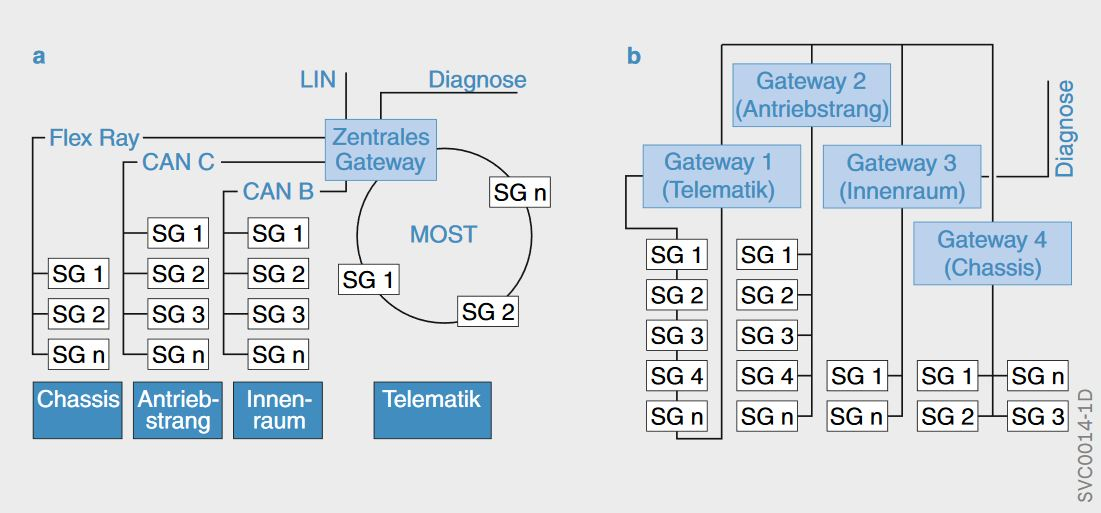
\includegraphics{Images/Kapitel3/TW01.JPG}
    \end{figure}
    
%\graphicspath{{./Images/Kapitel4/}}

\section{Bussysteme}

\subsection{Automotive Ethernet}
\subsubsection{Anwendung}
Für Ethernet im Automotive Bereich wird der Standard IEEE 802.3 verwendet. Trotz seiner hohen Beliebtheit und Verbreitung war Ethernet im Automotive Bereich lange Zeit undenkbar, vor allem da es keine Echtzeit erfüllen kann und für kleine Anwendungen zu teuer ist. Moderne Anwendungen (z.B. komplexere Assistenzsysteme, Diagnose- oder Multimedia-Anwendungen) fordern jedoch immer höhere Datenraten, so dass Ethernet immer mehr Beachtung bekommt. Es wurden auch Protokolle und Technologien entwickelt, um Ethernet besser an die Anforderungen anzupassen. Es gibt mit TimeTriggeredEthernet/SAE AS6802 einen echtzeitfähigen Ethernet Bus und durch Audio-Video-Bridging können komplexere Multi-Media-Anwendungen, z.B. Surround Sound oder synchrone Wiedergabe von Audio/Video-Dateien, realisiert werden. Um Kosten und Leitungen zu sparen wurde 100Base-T1 entwickelt, hier wird nur ein verdrillter Kupferdraht benutzt. \cite{.MH_Ethernet}

\subsubsection{Topologie}
Ethernet wird im Automotive Bereich oft in der Stern- (siehe Abbildung \ref{fig:stern}), Bus- (siehe Abbildung \ref{fig:bus}) oder Baumtopologie (siehe Abbildung \ref{fig:baum}) verwendet. Dies ist ein neuer Ansatz, da die meisten bisherigen Bussysteme nahezu nur auf die Stern- und Bustopologie setzen.

\cite{.MH_Vehicle}

\begin{figure}[h!]
	\centering
	\begin{subfigure}[b]{0.4\textwidth}
		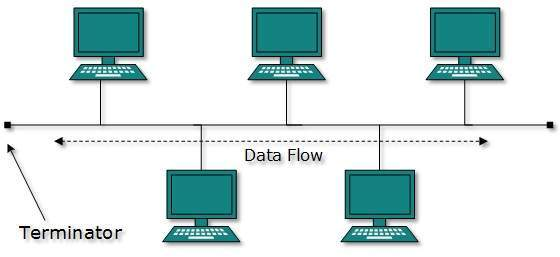
\includegraphics[width=\linewidth]{bus-topology.jpg}
		\subcaption[2.bp.blogspot.com/-R-uihxzRU6g/WOIFGLjqtMI/AAAAAAAAEdg/X3YgTGUxQ8MSCbm14OsABMnhWUTK-Ee-gCLcB/s1600/bus\textunderscore topology.jpg]{Bus}
		\label{fig:bus}
	\end{subfigure}
	\begin{subfigure}[b]{0.4\textwidth}
		\includegraphics[width=\linewidth]{stern-topology.jpg}
		\subcaption[slideplayer.org/slide/791365/2/images/3/Sternstruktur+(Ethernet+Twisted+Pair).jpg]{Stern}
		\label{fig:stern}
	\end{subfigure}
	\begin{subfigure}[b]{0.4\textwidth}
		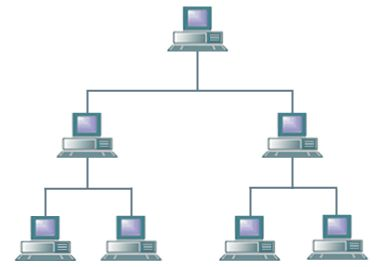
\includegraphics[width=\linewidth]{tree-topology.jpg}
		\subcaption[units.folder101.com/cisco/sem1/Notes/ch2-topologies/tree.gif]{Baum}
		\label{fig:baum}
	\end{subfigure}
	\caption{Ethernet Topologie}
\end{figure}

\subsubsection{Vor- und Nachteile}
\begin{tabular}{l|l}
	\textbf{Vorteile} & \textbf{Nachteile}\\
	\hline hohe Datenrate & hohe Kosten\\
	\hline neue Technologien z.B. Service discovery,  & keine Echtzeitfähigkeit, nicht\\
	DNS oder Streams für Multimedia & deterministisch\\
	\hline leichte Anbindung für IOT und Internet & Umdenken/Umdesignen für neue \\
	& Topologie und neuen Ansatz\\
	\hline viele Standardimplementationen und&\\
	Wiederverwertbarkeit der Software&\\
	\hline einfacher Austausch von Komponenten &\\
\end{tabular}

\subsection{MOST}		
\subsubsection{Anwendung}
Der MOST-Bus (Media Oriented Systems Transport) wird von der MOST Cooperation standardisiert und wird im Automotive Bereich nahezu ausschließlich für Multi-Media-Anwendungen eingesetzt. Durch seine hohe Datenrate kann es schnell viele Daten zwischen den Komponenten verschicken.


\cite{.MH_Vehicle}

\subsubsection{Topologie}
Ein MOST-Netzwerk ist immer als synchronisierter Ring aufgebaut (siehe Abbildung \ref{fig:ring}). Es gibt immer einen Master, der die Synchronisation steuert. Alle Komponenten haben eine Kontrollkanal, auf der Daten zum Status des Systems/Netzwerks gesendet werden. Zudem gibt es mehrere synchrone und asynchrone Kanäle, die sich die Bandbreite, je nach Last, teilen.
Auf dem synchronen Kanälen werden fortlaufende Daten, z.B. Audio- oder Videostreams verschickt.
Die asynchronen Kanäle sind für Daten reserviert, die nicht fortlaufend entstehen, aber schnell verarbeitet werden sollen. Z.B. Nutzereingaben zum Überspringen eines Songs oder Eingabe ins Navi. \cite{BP01}

\begin{figure}[h!]
	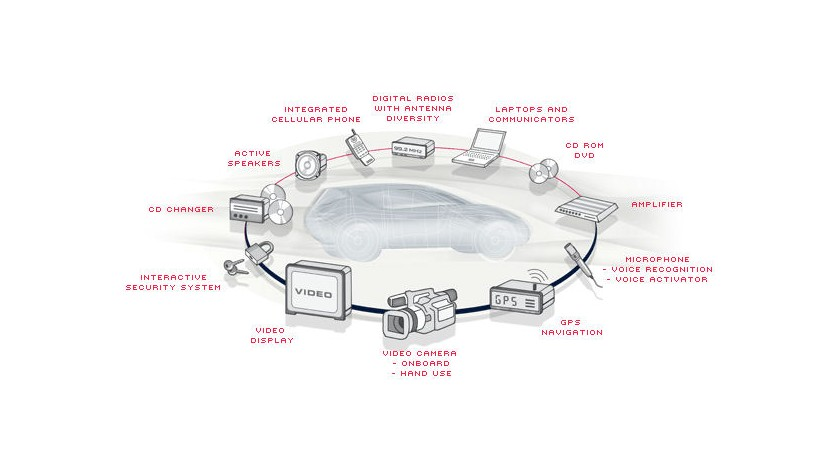
\includegraphics[width=\linewidth]{most-ring.jpg}
	%\caption[https://images.tecchannel.de/bdb/361603/840x473.jpg]{MOST Ring}
	\label{fig:ring}
\end{figure}

\subsubsection{Vor- und Nachteile}
\begin{tabular}{l|l}
	\textbf{Vorteile} & \textbf{Nachteile}\\
	\hline hohe Datenrate & hohe Kosten\\
	\hline einfacher Austausch von Komponenten & proprietäre Hardware\\
	\hline einheitliche Schnittstellen von Komponenten &\\
\end{tabular}

\subsection{Bluetooth}		
\subsubsection{Anwendung}
Bluetooth wird durch die Bluetooth Special Interest Group, ein Verband aus derzeit über 2000 Unternehmen,  standardisiert. Momentan ist Bluetooth 5 die aktuellste Version. Es wird im Automotive Bereich verwendet, um kostengünstige und kabellose Verbindungen aufzubauen. Der größte Bereich sind hierbei Multi-Media-Anwendungen, um beispielsweise Smartphones oder Kopfhörer anzubinden. \cite{BP01}

\subsubsection{Topologie}
Bluetooth Netzwerke haben immer einen Master, der die Kommunikation steuert. Dieser ist jedoch nicht fest, sondern wird erst beim Verbindungsaufbau ausgemacht.
Bluetooth-Netzwerke können entweder als Pico- oder Scatternet aufgebaut sein (siehe Abbildung \ref{fig:pico}).
                                                                                  
Ein Piconet ist eine Ansammlung von mindestens zwei Bluetooth-Geräten. Eines der Geräte übernimmt die Rolle des Masters und steuert die Kommunikation mit allen Slaves. Slaves können nur mit dem Master kommunizieren.

Ein Scatternet ist ein Zusammenschluss von mehreren Piconets, bei dem jeweils ein Knoten teil eines anderen Piconets ist. Dieser geteilte Knoten kann nicht gleichzeitig in beiden Netzen sein, sondern muss immer zwischen den Netzen wechseln. Der geteilte Knoten kann Master höchstens für eines der Netze sein.

\begin{figure}[h!]
	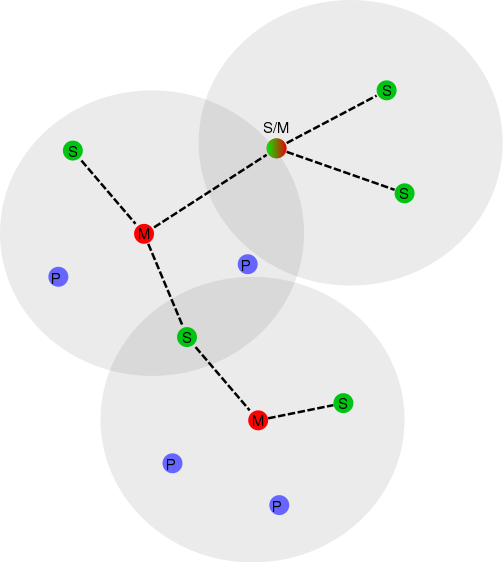
\includegraphics[width=0.7\linewidth]{pico-scatternet.png}
	%\caption[https://de.wikipedia.org/wiki/Scatternet#/media/Datei:BluetoothScatternet-de.svg]{Abbildung 4.5}
	\label{fig:pico}
\end{figure}

\subsubsection{Vor- und Nachteile}
\begin{tabular}{l|l}
	\textbf{Vorteile} & \textbf{Nachteile}\\
	\hline geringe Kosten & geringe Datenrate\\
	\hline kabellos & geringe Reichweite\\
	\hline Standardsoftware & störanfälliger als physische Busse\\
\end{tabular}


\graphicspath{{./Images/Kapitel5/}}
	
\begin{flushleft}
		
	\section{Sensoren}
		\subsection{Allgemeines} 
		
		Abbildung \ref{fig:TS01} zeigt eine grafische Übersicht der wichtigsten Sensoren in einem Fahrzeug:
				
		\begin{figure}[h!]
			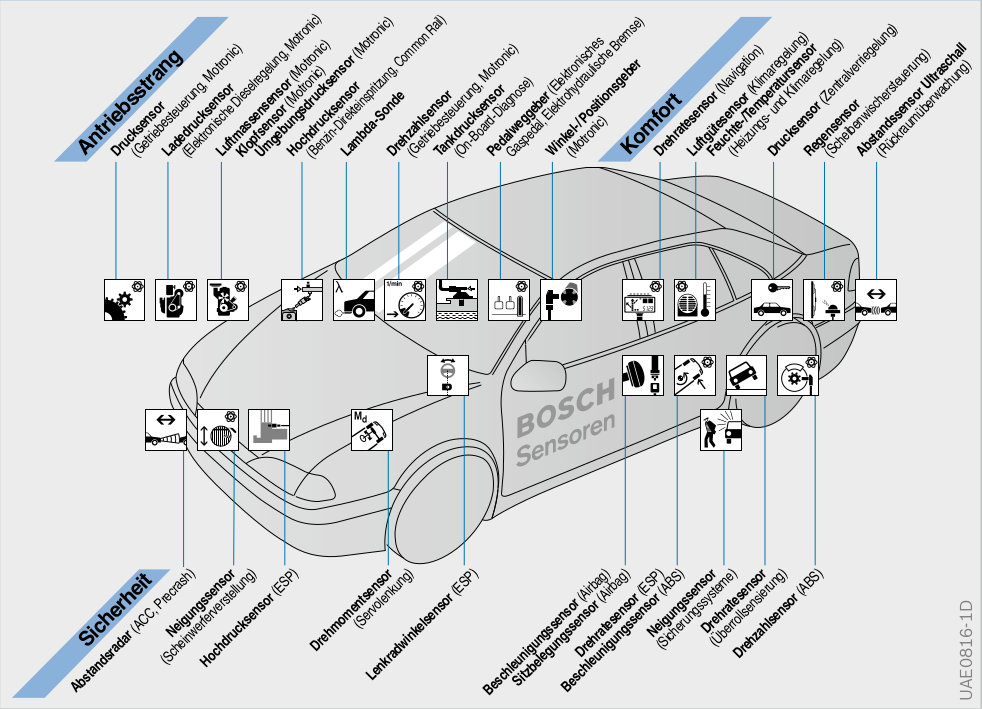
\includegraphics[width=\textwidth] {sensor_uebersicht.png}
	        \caption{Übersicht der Sensoren im Fahrzeug \cite{BP01}}
	        \label{fig:TS01}
		\end{figure}	
		
			\subsubsection{Begriffsdefinition}
		
	        Unter Sensor versteht man im allgemeinen eine
	        \begin{itemize}
	            \item Komponente
	            \item Fühler
	            \item Detektor
	            \item Aufnehmer
	        \end{itemize}
	            der eine physikalische Größe oder chemische Effekte durch messtechnische Verfahren aufnimmt und in ein analoges, elektrisches Strom- / Spannungssgnal umwandelt.
	        
	        \subsubsection{Arten von Sensoren \cite{TS_sensor_aufteilen}}
	
	        Grundlegend kann man zwischen mechanischen und nicht-mechanischen Sensoren unterscheiden. \\
	        \begin{itemize}
	            \item \textbf{Mechanische Sensoren}: verändern durch mechanische Einwirkungen von außen, zum Beispiel durch Kraft- oder Druckeinwirkung, ihre elektrische Eigenschaften.
	            \item \textbf{Nicht-Mechanische Sensoren}: verändern ihre Eigenschaften durch nicht-mechanische Einwirkungen, zum Beispiel chemisch durch Lichteinwirkung.
	        \end{itemize}
	        \begin{table}[h]
	        \begin{tabularx}{\textwidth}{l|l|l}
	
	                    \textbf{Sensorart} & \textbf{Messtechnik} & \textbf{Beispiele}\\
						\hline
	                    \multicolumn{3}{l}{\textbf{Mechanische Sensoren}}\\
	                    \hline
						Resistiv & Elektrische & Dehnungsmessstreifen \\
						&Widerstandsänderung& Potentiometrische Sensoren\\
						\hline
	                    
	                    Kapazitiv & Kapazitätsänderung & Drucksensor\\
	                    && kapazitiver Näherungsschalter \\
						\hline
						
						Temperatur & Kontaktthermometrie & Thermoelement\\
						&& Widerstandsthermometer \\
	                    \hline
	
	                    \multicolumn{3}{l}{\textbf{Nicht-Mechanische Sensoren}}\\
	                    \hline
	
	                    Induktiv & Änderung der Induktion & Schwingungsaufnehmer \\
	                    && Induktivaufnehmer\\
	                    \hline
									
	                    Wirbelstrom & Änderung des Wirbelstroms & Induktive Initiatoren\\
	                    \hline
	                    
	                    Magnetfeld & Änderung des Magnetfelds & Hall-Generator\\
	                    && Feldplatte\\
	                    \hline
	
	                    Optoelektisch & Änderung der Lichtstärke & Fototransistor\\
	                    && Fotodiode\\
	                    
	
	                \end{tabularx}\\
	                \caption{Arten von Sensoren}
	                \label{fig:TS09}
	            \end{table}
	         	
	                	Desweiteren wird zwischen aktiven und passiven Sensoren unterschieden. 
	                	
	                	Ein aktiver Sensor ist selbst ein Spannungserzeuger und benötigt keine weitere elektrische Hilfsenergie, um betrieben zu werden. Beispiele dazu wären ein Thermoelement, Licht- oder Drucksensor.\\
	                	
	                	Passive Sensoren hingegen benötigen eine aktive Spannungsversorgung, auch Sekundärelektronik genannt, welche es erlaubt, die Messung in elektrische Signale, also in Primärelektronik, umzuwandeln. Beispiele dazu wären eine Wägezelle, Dehnungsmessstreifen, Magnetfeldsensoren.		
	                	
	                                        
	\subsection{Klassische Sensoren im Automobil} 
	       
	    Nach dieser allgemeinen Grobeinteilung von Sensoren, soll nun im Weiteren spezieller auf die Sensortechnik in Kraftfahrzeugen eingegangen werden.
	
	    Der Grund für die immer umfangreichere Sensortechnik in Automobilen liegt in der Veränderung des Automobils im Laufe der Zeit, insbesondere im Hinblick auf Fahrunterstützung und Fahrhilfssysteme.
	     	
	    Die Sensoren dienen hierbei der Eingabe,  bzw. dem Auslesen eines tatsächlichen Wertes (Ist-Wert). Diese werden einer ECU über ein Bussystem übermittelt, welches einen Abgleich des Ist-Wertes mit einem vorgegebenen Soll-Wert vornimmt und dementsprechend das Modul nachregeln und steuern kann. \\ 
	    
	    Da Sensoren diversen äußeren physikalischen und/ oder chemischen Einwirkungen ausgesetzt sind, müssen sie diesen entsprechend gerecht werden. Aus diesem Grund gibt es verschiedene Anfertigungsformen wie wasserdicht, dreck- und staubgeschützt. Diese werden in dem nächsten Kapitel ebenfalls erörtert.\\  
	            
	    Ein Ausfall des Sensors kann durch folgende Ursachen hervorgerufen werden:
	
	        \begin{itemize}
	            \item Kurzschlussbeginn
	            \item Leitungsunterbrechung
	            \item Verschmutzung
	            \item Mechanische Beschädigung
	            \item nicht korrektes Anbringen des Sensors
	            \item Sensor defekt
	        \end{itemize}	
	        
	        Nach einem Ausfall kann man durch gezielte Fehlersuche der Fehler analysiert werden:
	
	        \begin{itemize}
	            \item Anschlüsse prüfen
	            \item Auslesen des Fehlerspeichers
	            \item Allgemeine optische Prüfung
	            \item Säubern der Sensoren
	            \item Messungen mit einem Messinstrument vornehmen wie:
	            \begin{itemize}
	                \item Oszilloskop 
	                \item Voltmeter
	                \item Amperemeter
	                \item Ohmmeter	
	            \end{itemize}
	            
	        \end{itemize}
	
			In den nachfolgenden Beschreibungen sind einige, in Abbildung \ref{fig:TS01} dargestellte Sensoren, zusammengefasst, da die Funktionsweise mancher Sensoren sehr ähnlich sind.
			
	        \subsubsection{Temperatursensor NTC}
				Bei einem Temperatursensor handelt es sich um einen nicht-mechanischen, aktiven	Sensor, welcher die Temperatur erfasst.\\
	            Die Sensoren sind auf einen Messbereich zwischen -40$^\circ$C und +200$^\circ$C skaliert.
	            Für Temperaturen, die über diesen Bereich herausgehen, werden spezielle Hochtemperatursensoren (HTS) verwendet.
	
	            \begin{figure}[h]
				
		        	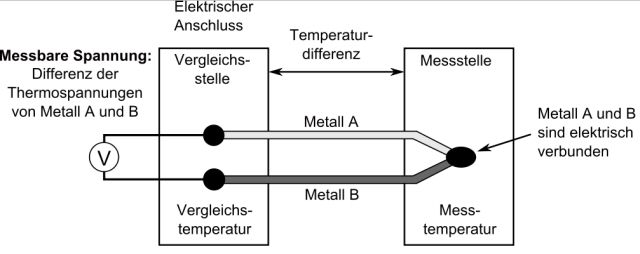
\includegraphics[width=\textwidth]{aufbau_ntc.png}
		            \caption[www.kfztech.de/kfztechnik/elo/sensoren/ntc.htm]{Aufbau NTC}
		            \label{fig:TS02}
	            
				\end{figure}
	
	            Abbildung \ref{fig:TS02} zeigt den Aufbau eines Temperatursensors.
	
	            Hierbei werden zwei unterschiedlich, elektrisch aufgeladene Metalle am Ende (der Messstelle) miteinander verbunden. Hier wird die Temperatur von dem zu messenden Element gemessen.\\
	            Die Temperaturdifferenz wird an den zwei offenen Enden mit Hilfe des Seebeck-Effekts in elektrische Spannung umgewandelt. 
	            Dann kann die Differenz der beiden Leiter verglichen werden, wobei einer der Leiter als Referenz benutzt wird (grauer Leiter).\cite{TS_temp} 
						
				NTC Sensoren werden beispielsweise in folgenden Komponenten verwendet:
				
				\begin{itemize}
					\item Katalysator
					\item Öltemperatur
					\item Klimaanlagen
					\item Kühlwassertemperatur 	
				\end{itemize}
				
	            HTS hingegen werden für
	            
				\begin{itemize}
					\item AGR
					\item Turbolader
					\item Rußfilter 
	            \end{itemize}
	            
	            eingesetzt.
	
	            \subsubsection{Induktive Sensoren}
			
	            Induktive Sensoren arbeiten nach dem Induktionsgesetz.
	            
				Hierbei erleidet der Sensor keinerlei Verschleiß, da kein direkter Kontakt zu dem zu messenden Objekt existiert.\\
				Für ein Verständnis, wo diese Sensoren welche Aufgaben im KFZ- Bereich erfüllt, reicht es nur den groben Aufbau zu kennen.\\
				Eine Spule wird von Strom durchflossen, welche daraufhin ein Magnetfeld erzeugt.\\	
	
				\begin{figure}[h]
					\centering
					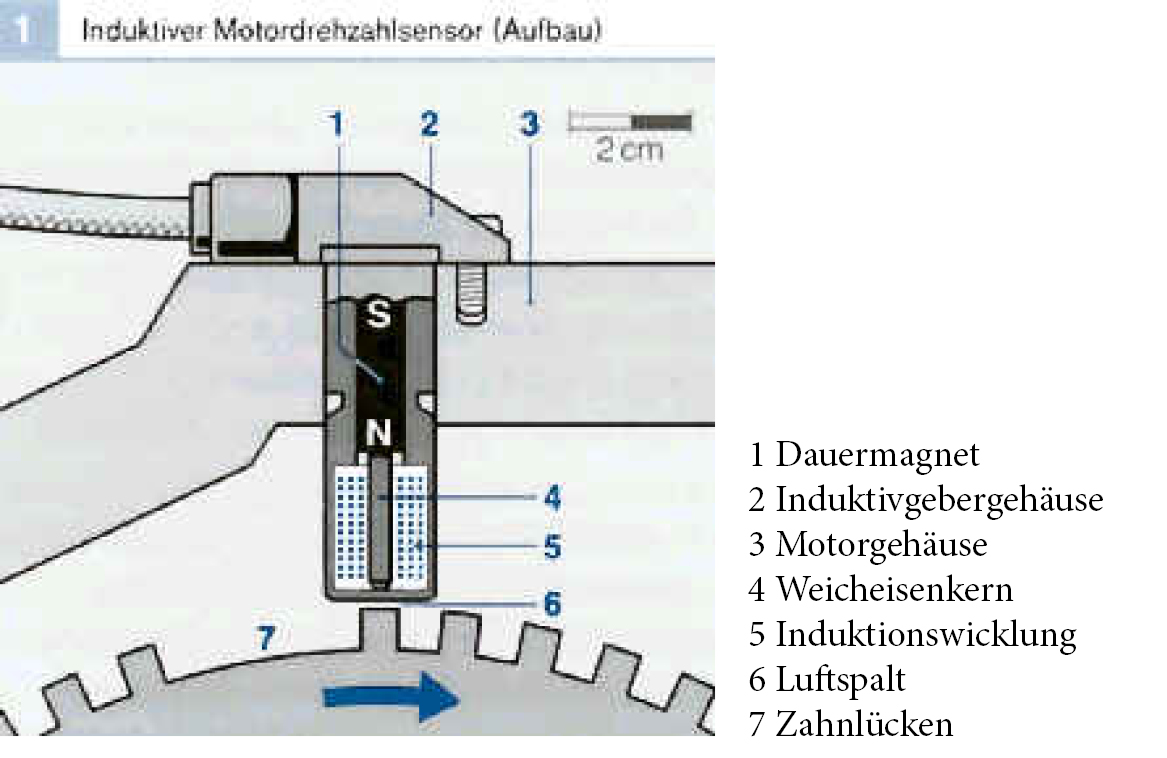
\includegraphics{Induktiv_mit_legende.jpg}
					\caption[www.kfztech.de/kfztechnik/elo/sensoren/induktivgeber.htm]{Induktiver Sensor}
					\label{fig:TS03}
				\end{figure}
				
				In Abbildung \ref{fig:TS03} ist der Sensor über einer Art Zahnrad, welches man Impulsrad nennt, angebracht.\\
	            
	            "Der magnetische Fluss durch die Spule hängt davon ab, ob dem Sensor eine Lücke oder ein Zahn gegenübersteht. Ein Zahn bündelt den Streufluss des Magneten, eine Lücke dagegen schwächt den Magnetfluss." \cite{TS_ind_funkt}  
				Die Anzahl der Änderungen/ Impulse in einer bestimmten Zeiteinheit ist ein Maß für die Drehzahl des zu messenden Objekts. Darüber hinaus kann auch die exakte Position des Moduls erkannt werden.\\					
	            
				Induktive Sensoren werden beispielsweise in folgenden Modulen verwendet:
				
				\begin{itemize}
					\item Drehzahlerfassung wie
						\begin{itemize}
							\item Kurbelwellenstellung
							\item Getriebe
						\end{itemize}	
					\item Drosselklappenstellung
					\item Lenkwinkel z.b. ESP
					\item Fahrpedalgeber
					\item Bremspedal
				\end{itemize}
			
				Allerdings kann der Ausfall eines Sensors zu erheblichen Schäden und sicherheitstechnischen Gefährdungen führen:
				\begin{itemize}
					\item Motor kann aussetzen oder gar stillstehen
					\item es wird ein Fehlercode abgespeichert
	            \end{itemize}
	           
	          
	           \subsubsection{Luftmassenmesser}
	           
	            Der Sensor misst im Prinzip die Luftmasse pro eingestellter Zeitspanne. Da der Massenstrom in einem bestimmten Verhältnis, meist proportional, zu dem enthaltenen Sauerstoffgehalt ist, kann dies zur Regularisierung des Verbrennprozesses im Motor beisteuern.
	           
	            \subsubsection{Ölsensor}
						
	            Dieser Sensor wird verwendet, um Informationen über den Zustand und den Füllstand des Öls zu erhalten. So kann angezeigt werden, ob und wann ein Ölwechsel notwendig ist. 
	            Das Einbringen des Ölsensors spart also Geld, schont die Umwelt und gibt Rückschlüsse auf den Zustand des Motors und es können Motorschäden verhindern.\cite{TS_oel}
	            
	            \subsubsection{Lenkdrehmomentsensor}
	
	            ``Um die Funktion des Servomoduls umsetzen zu können, benötigt das Steuergerät exakte Informationen über die vom Fahrer eingegebene Lenkbefehle. Um diese Eingabe richtig erfassen zu können, wurde ein Sensor konstruiert, welcher [...] die erforderlichen Daten wie Drehwinkel, Drehrichtung und Drehmoment elektronisch erfassen.[...] ``  \cite{TS_dreh} kann und an das Steuergerät sendet.\\
	            
	            Die Funktionsweise eines Drehmomentsensors kann auf zwei Arten realisiert werden:\\
	            
	            \begin{enumerate}
	                \item \textbf{Magnetoresistives Prinzip}:
	                
	                         Mittels Eingangswelle, Torsionsstab/ Drehstab (eine stabförmige Feder, welche sich in axialer Richtung drehen lässt), Antriebswelle und einem magnetoresistivem Element. \\
	                         Damit Leitungen zur Spannungsversorgung und Signalübertragung nicht beschädigt werden, sind diese in einer Vermantelung, welche auch als Wickelkassette bezeichnet wird.\\
	                         
	                         Durch das Einlenken des Fahrers wird der Torisonsstab ebenfalls verdreht. ``Diese Verdrehung ist ein Maß für das Lenkmoment.`` \cite{TS_dreh}
	
	                         Durch gezieltes Aufbringen von Widerständen können die Drehbewegungen registriert werden. Durch das Drehen, also spannen oder stauchen der Feder ( Fahrer lenkt links bzw rechts ein) verändert sich das Magnetfeld, welches wiederum den elektrischen Widerstand verändert und somit die über dem Widerstand anliegende Spannung. Diese Spannungssignale werden über die Signalleitungen an das Steuergerät übersendet, welches aus den Informationen die aufzubringende Unterstützungsmomente berechnen kann.				 
	
	                \item \textbf{Optisches Prinzip}:\\
	
	                        Vor und hinter dem Torsionsstab ist jeweils eine Scheibe angebracht, welche eine bestimmte Codierung mittels eingelassenen Löchern hat (siehe Abbildung \ref{fig:TS05}).\\
	                        Zur Bestimmung der Einlenkgeschwindigkeit wird axial und parallel zu dem Torsionsstab eine Leuchtdiode (über der ersten Scheibe) und eine Fotodiode (unter der zweiten Scheibe) angebracht. \\
	                        Die Leuchtdiode sendet gebündeltes Licht aus, welches auf der gegenüberliegenden Seite von der Fotodiode erkannt wird. Bei einfallendem Licht verändert sich der durchfließende elektrische Strom durch die Fotodiode.\\
	                        Dreht sich also die Scheibe kommt es zu einem Wechsel der Stromstärke. Diese Impulse werden an das angebundene Steuergerät gesendet, welches aus diesen empfangenden Informationen die Drehgeschwindigkeit berechnen kann.\\
	                        
	                        \begin{figure}[h]
	                            \centering
	                            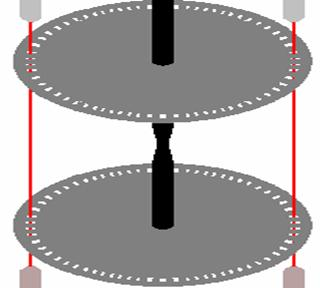
\includegraphics{photoelektrisch.png}
	                             \caption[www.kfztech.de/kfztechnik/fahrwerk/lenkung/photoelektrisch.jpg]{Photooptisches Prinzip}
	                             \label{fig:TS05}
	                        \end{figure}	
	            \end{enumerate}
	
	            \subsubsection{Regensensor}
	
	                Dieser nicht-mechanische Sensor ``[...] registriert Wassertropfen auf der Windschutzscheibe durch opto-elektrisches Verfahren`` \cite{TS_regen}
	                
	                Der Regensensor befindet sich innerhalb des Wischbereichs des Scheibenwischers.                
					In dem Sensor befindet sich eine Leuchtdiode und eine Fotodiode, welche in einem bestimmten Abstand voneinander angebracht sind. Die Leuchtdiode sendet ein Infrarotlicht aus. Dieses Lichtbündel wird bei trockener Windschutzscheibe an der äußeren Scheibe reflektiert und nahezu mit voller Lichtstärke von dem Sensor aufgenommen. In der Physik spricht man hier von einer Totalreflexion.\\
					Befinden sich nun Wassertropfen in dem Bereich des Sensors auf der Frontscheibe wird das ausgesendete Lichtbündel nicht komplett reflektiert, sondern ein Teil des Lichtes wird gebrochen und durch den Tropfen gestreut. Das Resultat daraus ist, dass der ausgesendete Lichtstrahl nur noch mit einem Bruchteil der ursprünglichen Stärke den Sensor erreicht.\\
					Aus diesen Daten errechnet die dort darin befindliche Elektronik die Stärke des Niederschlages, gibt diese an ein Steuergerät weiter, welches wiederum die Scheibenwischer ansteuert. Somit bleibt die Oberfläche des Sensors immer tropfenfrei und es wird ein optimales Messergebnis erreicht. (Fig. 8)
					
					\begin{figure}[h]
						\centering
						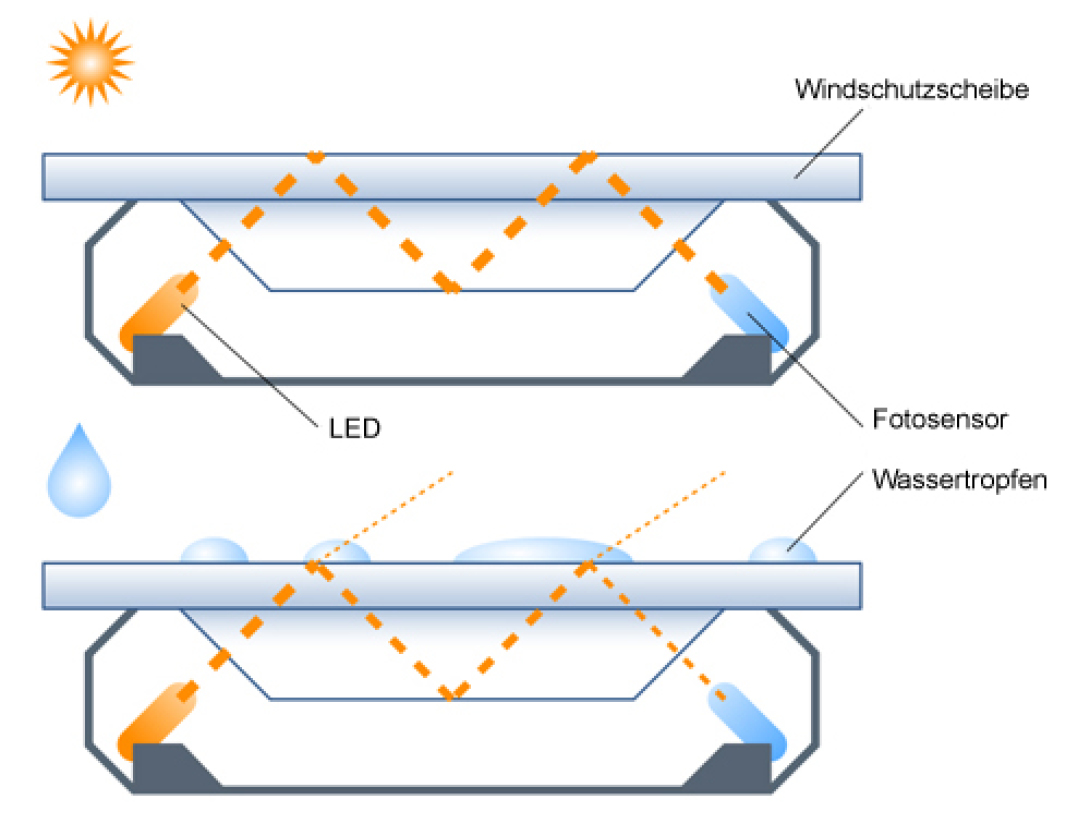
\includegraphics{regensensor2.jpg}
	                    \caption[archiv.langzeittest.de/volvo-s40/intern/grafik/cb-regensensor-prinzip.jpg] {Prinzip eines Regensensors}
	                    \label{fig:TS06}
	                \end{figure}
	                
	            \subsubsection{Seitenwandtorsionssensor}
	
					Elektronische Regelsysteme wie ABS oder ESP benötigen sämtliche Informationen über das Zusammenspiel zwischen Fahrzeug und dem Fahruntergrund und den daraus entstehenden Kräften. Um die einzelnen Sekundärgrößen wie Motorleistung, Bremsdruck, Radgeschwindigkeit und Fahrzeugbeschleunigung zur Berechnung nicht mehr benutzen zu müssen, wurde von Continental ein Sensorsystem entwickelt, welches das Rad als Sensor fungieren lässt, das sogenannte SWT-System. 
					
					\begin{figure}[h]
						\centering
						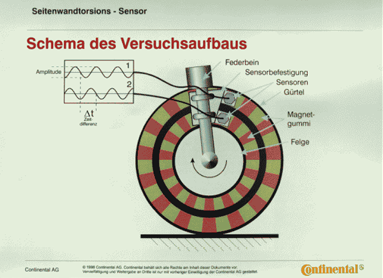
\includegraphics{swt1.png}
	                    \caption[www.kfztech.de/kfztechnik/sicherheit/swt/swt1.gif]{Reifen als Sensor}
	                    \label{fig:TS07}
					\end{figure}
				
	                Der Reifen besteht aus Magnetgummi und Magnetfeldsensoren, sowie einem Signalaufbereitungssystem und einer zentralen Recheneinheit.
						
	                Die Messung findet mittels der Verformung des Reifens statt, die entsteht wenn der Reifen bei Kurvenfahrten durch die einwirkenden Querkräfte temporär aus der Form gebracht wird. 
	                
	                Hierfür werden zwei Sensoren am Fahrwerk angebracht, wobei einer der beiden auf der Höhe der Felge ist und der andere nahe am Scheitelpunkt des Reifens angebracht wird. Darüber hinaus ist die Reifenseitenwand magnetisch, um ein Messergebnis erzielen zu können.\\
	                In der obrigen Abbildung erkennen wir ein Muster auf dem Reifen. Dies ist darauf zurückzuführen, dass ein Magnetpulver in die Reifenseitenwand eingemischt wird. Dieses Gemisch wird über den gesamten Umfang des Reifens gestrichen und somit erhält man eine alterniernde Nord- und Südpole, was durch die Streifen visualisiert wird.
	                
	                Solange auf den Reifen keine Längskräfte wirken, ``[]...] erfolgt der Wechsel zwischen den Magnetpolen an beiden Sensoren gleichzeitig, die Zeitdifferenz zwischen den Signalen beider Sensoren ist Null`` \cite{TS_swt} \\	
	                Beschleunigt oder verzögert der Fahrer das Fahrzeug, überschreiten die Grenzen der Magnete zu unterschiedlichen Zeiten die Sensoren, somit ist eine Zeitdifferenz zu messen. 
	                Diese gemessene Zeitdifferenz wird an ein eingebautes Steuergerät gesendet, welche die Fahrassistenzsysteme wie ASR und ABS anspricht und dementsprechend der derzeitigen Fahrsituation anpasst.\\
	                
					Während einer Kurvenfahrt kann der Abstand zwischen der Reifenseitenwand und dem Sensor gemessen werden, da sich dieser mechanisch gesehen verkürzt bzw. vergrößert wird und sich somit die Stärke des Magnetfelds ändert.\\
	                Mit Hilfe dieser gemessenen Werten können Hilfssysteme wie ASB und ESP entsprechend angesteuert werden. Dies sorgt für ein sichereres Fahren da die Ansteuerung optimiert werden kann. 
	                
	                In der Praxis bedeutet dies, dass der Fahrer einen kürzeren Bremsweg und eine bessere Kontrolle über das Fahrzeug auf kurvenreichen und schweren Strecken hat.
	
	                \subsubsection{Reifensensor}
	
	                Ein in den Reifenprofil eingebetteter Chip überträgt hochfrequent die Signale an eine im Radkasten befindliche Antenne. 
	                Ändert sich der Zustand der Straße verändert der Sensor das Signal. Dies geschieht pro Sekunde mehrere Male. 
	                Darüberhinaus kontrolliert der Sensor permanent den Reifendruck. Mit diesen Informationen kann nicht nur die Lebensdauer des Reifens, sondern auch die Sicherheit erhöht werden, 
	                da sich gezielt ABS und ESP einschalten.\\ 
				
	                \subsubsection{Reifendrucküberwachungssystem}
	                Reifendrucküberwachungssysteme (RDKS) werden eingesetzt, um die Lebensdauer des Reifens zu erhöhen. Seit 1. November 2014 sind die Reifen- und Autohersteller verpflichtet, ein RKDS zu implementieren.
	                Hierbei wird jeder Reifen mit einem Sensor ausgestattet, damit der Fahrer Luftverlust oder gar einen Plattfuß bemerken kann.
	                
	                Prinzipiell gibt es RDKS in aktiver und passiver Variante. In Tabelle \ref{fig:TS08} werden diese in Funktionsweise mit ihren jeweiligen
	                Vor- und Nachteilen gegenübergestellt.
	
	                \begin{table}
	                    \begin{tabularx}{\textwidth} {l|l}
	                        
	                        
	                        \multicolumn{2}{c}{\textbf{Passives Reifendrucküberwachungssystem}}\\
	                        \hline
	                        \textbf{Erklärung:} & Platter Reifen hat einen kleineren Abrollumfang \\ & und dreht sich schneller.\\ & ABS Sensoren messen dies und das Steuergerät erkennt dies\\
	                        \hline
	                        \textbf{Vorteil:} & kostengünstig, in Kombination mit Runflat Tyres eine \\ & optimale Lösung, da nur eine geänderte Software \\ & und Kontrolle erforderlich sind.\\
	                        \hline
	                        \textbf{Nachteil:} & schleichender Luftverlust der Räder an einer Achse \\ &  wird nicht erkannt. Nur Differenzen größer 0.5 Bar werden \\ & während der Fahrt erkannt. Höherer Spritverbrauch durch \\ & zu niedrigen Luftdruck.\\
	                        \multicolumn{2}{c}{\textbf{Aktives Reifendrucküberwachungssystem}}\\
	                        \hline
	                        \textbf{Erklärung:} & Jeder Reifen besitzt eigenen Sensor und sendet Informationen \\ & über Druck und Temperatur per Funk an Steuergerät.\\
	                        \hline
	                        \textbf{Vorteil:} & Exakte Messung, ab einer Differenz von 0.2 Bar wird ein \\ & Alarm ausgelöst. Reserverad wird mit überwacht.\\
	                        \hline
	                        \textbf{Nachteil:}  & Teuer für Reifenmontage, da Reifen kodiert werden müssen\\ & und der Reifenwechsel aufwendig wird.\\
	
	                    \end{tabularx}
	                    \caption{Aktive und Passive Reifendrucküberwachungssysteme \cite{TS_rdks}}
	                    \label{fig:TS08}
	
	                \end{table}
	
	                
	                Die Reifenelektronik sitzt auf der Innenseite des Reifen und misst in kurzen definierten Zeitabständen Reifendruck und Temperatur. 
	                Jeder Sensor ist mit einer eigenen ID- Nummer ausgestattet. Per Funk werden an die eigene Empfangsstation Datenpakete geschickt, welche die ID, sowie Druck und Temperatur des Reifens beinhalten.
	
	                Dieses Empfangsgerät sendet die empfangenen Daten kabelgebunden weiter an das Steuergerät. Dieses wertet die Daten aus und sendet bei Bedarf, sprich Unter- oder Überschreitung der Sollwerte, eine Meldung an die Kontrollanzeige.
					
	                \subsubsection{Hallsensor}
	
					Hallsensoren werden eingesetzt in: 
					\begin{itemize}
						\item Zündanlage
						\item Getriebeausgabedrehzahl
						\item Radlöseerkennung/- warnung (Audi)
						\item aktiver Drehzahlsensor in ABS- Bremsanlagen
						\item Nockenwelle (Koordination von Eispritzungsbeginnberechnung oder Pumpe-Düse, sowie Klopfregelung)
					\end{itemize}
					
	                Am Beispiel des Nockenwellensensors wird im Folgenden die Funktion des Sensors beschrieben.
	                
	                Die Nockenwelle bringt einen aus ferromagnetischem Material angefertigten Rotor zum Drehen. Zwischen Rotor und einem Dauermagnet befindet sich der Sensor.
	                Durch den Dauermagneten wird ein Magnetfeld erzeugt, welches den Sensor senkrecht durchfließt. Passiert ein metallischer Gegenstand, beispielsweise ein Zahn der Nockenwelle, verändert dieser das Magnetfeld, welches den Sensor durchfließt.
					Elektronen werden senkrecht zum Magnetfeld stärker abgelenkt, wobei eine Hall-Spannung von mehreren Millivolt erzeugt. Eine integrierte Auswerteelektronik bereitet das Signal auf und leitet es an in Form eines Rechtecksignals an das Steuergerät geleitet. \cite{TS_hall}
	
					\begin{figure}[h]
						\centering
						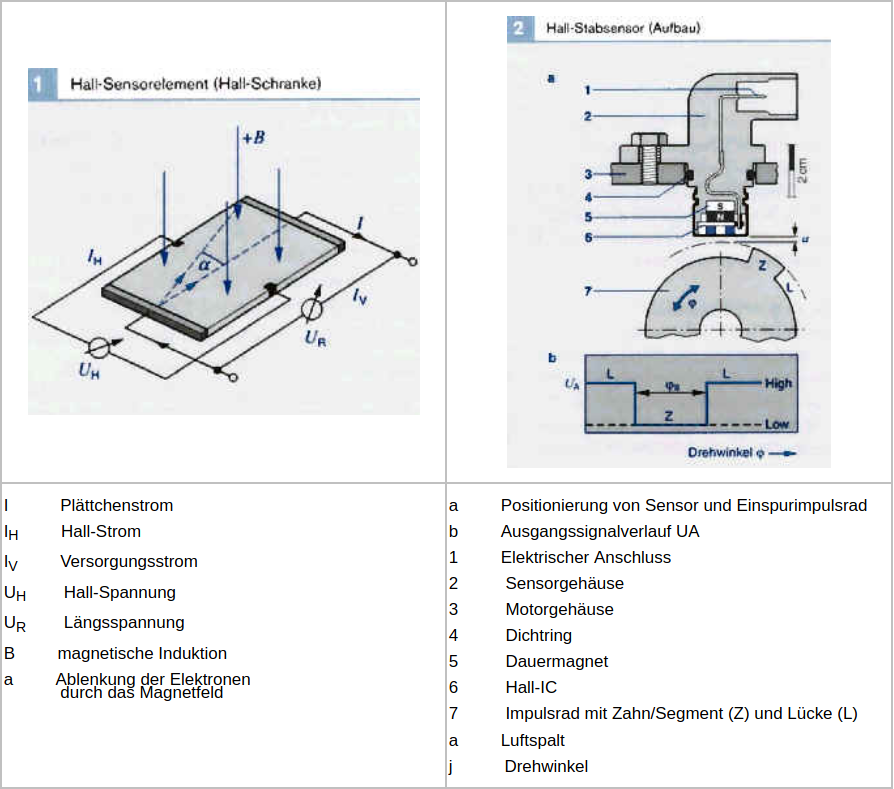
\includegraphics[width=\textwidth]{hall.png}
						\caption[www.kfztech.de/kfztechnik/elo/sensoren/hallsensor.htm]{Aufbau eines Hall-Sensors}
	                \end{figure}
	                
	                \subsubsection{Drehzahlsensor}
	
					Durch drei entsprechend angeordnete Sensoren kann die Drehrichtung des Rades erkannt werden. Ein entsprechend angeordneter Magnet (Abbildung \ref{fig:TS10}) ersetzt hierbei die Funktion der mechanischen Zahnräder.\\
	                \textbf{Aktive Sensoren}: Dieser wird bereits mit Spannung versorgt und erzeugt aus dem wechselnden Magnetfeld ein Rechtecksignal und sendet diese unverändert an ein Steuergerät.
	                
					Dies ermöglicht ebenso eine Geschwindigkeitsmessung von 0.1km/h. Diese Werte kann man zum Beispiel für Einparksysteme oder Navigationssysteme benutzen.\cite{TS_drehzahl_sensor}
					(Abbildung \ref{fig:TS11})
	
	                \begin{figure}[h!]
	                    \begin{minipage}[b]{.4\linewidth} % [b] => Ausrichtung an \caption
	                       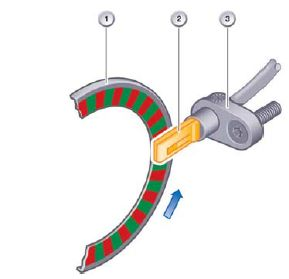
\includegraphics[width=\linewidth]{radsensor.png}
	                       \caption{Aufbau}
	                       \label{fig:TS10}
	                    \end{minipage}
	                    \hspace{.1\linewidth}% Abstand zwischen Bilder
	                    \begin{minipage}[b]{.4\linewidth} % [b] => Ausrichtung an \caption
	                       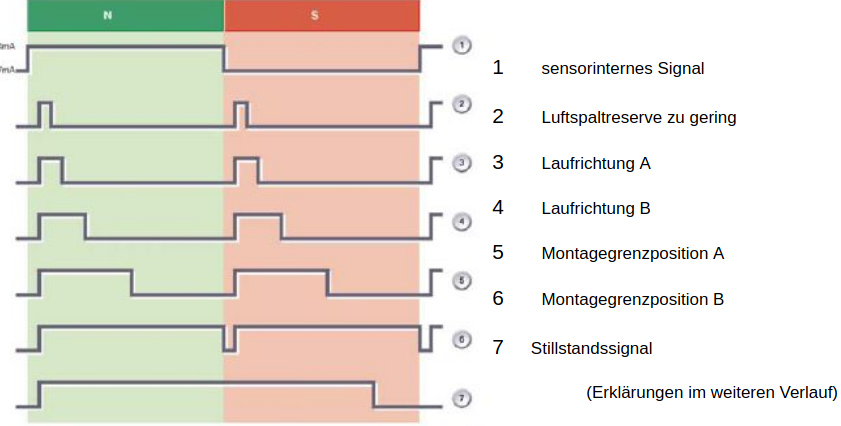
\includegraphics[width=\linewidth]{signalverlauf_hall.png}
	                       \caption[www.kfztech.de/kfztechnik/elo/sensoren/drehzahlsensor.htm]{Signalverlauf}
	                       \label{fig:TS11}
	                    \end{minipage}
	                 \end{figure}
	
	                 \subsubsection{Airbagsensor}
	
	                 Für das Auslösen des Airbags werden mehrere Frontsensoren verwendet, welche an diversen Stellen im Auto angebracht sind. Die Beschleunigungssensoren messen einwirkende Kräfte und geben ein Signal an das Steuergerät.
	                 Damit der Airbag nicht fälschlicherweise geöffnet wird, muss ein Sicherheitssensor innerhalb des Steuergerätes dies bestätigen. 
	                 
	                 ``Durch das genau Erfassen der Unfallschwere wird die Auslösung der Airbags und der Gurtstraffer aktiviert.`` \cite{TS_airbag}\\
	                 Faktoren sind: 
	                 
	                 \begin{itemize}
	                     \item Aufprallstärke
	                     \item Sicherheitsgurte angelegt
	                     \item Sitzposition des Fahrers und Beifahrers
	                 \end{itemize}
	             
	             
	             \subsubsection{Positionssensoren}
	
	                 Diese Sensoren sind an diversen relevanten Stellen des Automobils befestigt. Sie geben Aufschluss über Gegenstände in unmittelbarer Nähe des Fahrzeug.
	
	                 Um diese erkennen zu können wird ein Ultraschallsensor eingesetzt, welcher ein Signal aussendet. Falls ein Gegenstand in der Nähe ist, reflektiert dieser die Schallwellen und ein Ultraschallempfänger empfängt diese. 
	                 Durch die Zeitdifferenz des ausgesendeten und des erhaltenen Signals kann die Entfernung errechnet werden. Kommt das Objekt näher, so verkürzt sich der Abstand und somit auch die Zeit des Eintreffen des Schalls.
	
	                 Der Sensor sendet zu einen die Zeit, wann dieser die Ultraschallwellen gesendet hat sowie die reflektierten Signale. Aus dieser Differenz kann  der Abstand zwischen Auto und Gegenstand errechnet werden. 
	                 Nähert sich das Auto einem Objekt, so verkürzt sich die Zeit zwischen den austretenden und empfangenen Schallwellen. Bei dem kleinsten zulässigen Abstand meldet das Steuergerät dies der Kontrolleinheit und der Fahrer wird informiert.
	
	                 Falls sich kein Objekt in der Nähe befindet wird auch kein Signal reflektiert und somit erkennt das Steuergerät, dass keine Kollision stattfinden kann.
	
	                \subsection{Smarte Sensoren} 
	                 Unter smarten Sensoren versteht man Sensoren, die über eine integrierte Recheneinheit und -logik verfügen.
	                 
	                 Dadurch können diese Sensoren neben dem reinen Messen die eingelesenen Daten direkt verarbeiten und in diesem Zustand dem Steuergerät überreichen. 
	                 
	                 Dies hat den Vorteil, dass das Steuergerät keine überflüssigen Rechenschritte abarbeiten muss und somit mehr Rechenleistung für die Reaktion auf besondere Ereignisse hat.
	
	                 Smarte Sensoren können beispielsweise bei Feldbussystemen wie LIN, CAN, Flexray eingesetzt werden.		
	             	             
	             
	             \subsection{Zukunftsvisionen} 
	                  Durch das Weiterentwickeln der Sensortechnik können beispielsweise Unfälle vermieden werden, da der Sensor eine deutlich schnellere Reaktionszeit aufweist als ein Mensch.
	                  Ein Beispiel wäre, das bestehende Positionssensorsystem durch eine neue Art der Messung zu ersetzen. Hierbei werden die Ultraschallsensoren 
	                  durch sogenannte Radarkameras ersetzt, welche einen deutlich weiteren Radius abdecken können, als die bisher herkömmlichen Sensoren.(Fig. 18)
	                  
	                  \begin{figure}
	                      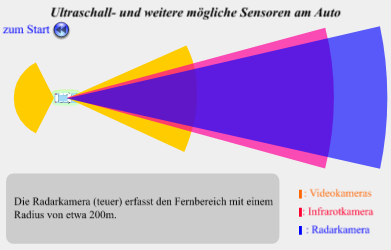
\includegraphics[width=\textwidth] {radarsensor.png}
	                      \caption[www.leifiphysik.de/akustik/schallgeschwindigkeit/ausblick/ultraschall-beim-auto]{Unterschied: Video-, Infrarot- und Radarkamera}
	                      \label{fig:TS12}
	                  \end{figure}
	     
	                     In Abbildung \ref{fig:TS12} kann man deutlich den Unterschied in der Reichweite der verschiedenen Sensoren sehen.\\
	                     
	                     Neben diesem Effekt kann durch neue entwickelten Sensoren beispielsweise der Spritverbrauch und somit den Ausstoß an $CO_2$ verringert werden.\\
	                     Auch im Hinblick auf Elektromobilität wird es neue Sensoren geben, welche zur Überwachung der Batterie eingesetzt werden.
\end{flushleft}
%\section{ECU / Steuergeräte}
Test
%\section{Fahrerassistenzsysteme}
    \subsection{Einführung}
    Fahrerassistenzsysteme sind Systeme die elektrisch den Autofahrer in bestimmten
    Situationen helfen und unterstüzen. Je nach Marke, Modell und Land können
    unterschiedliche Kombinationen von Fahrerassistenzsysteme hinzugebucht werden
    oder sind als Standardequipment bereits im Fahrzeug eingebaut. Solche Assistenten
    werden für die Sicherheit und den Komfort in die Automobile eingebaut. Für die
    einzelnen Systeme werden verschiedene Geräte wie Sensoren, Radar, Video oder
    Ultraschall verwendet, um ausreichend Informationen für die einzelnen Assistenten
    zu bekommen. Wenn nun eine riskante Situation aus der Sicht der Systeme entsteht,
    wird diese dem Fahrer durch visuelle und akustische Signale mitgeteilt. Solche
    Fahrerassistenten ersetzen bei manchen Stellen komplett den Fahrer und dies ist
    der Weg zum Autonomen Fahren.
    ~\cite{assistenzsysteme.PB1} ~\cite{assistenzsysteme.PB2} ~\cite{assistenzsysteme.PB3}
    ~\cite{assistenzsysteme.PB4}
    \subsection{Fahrerassistenzsysteme}

        \subsubsection{Antiblockiersystem (ABS)}
        ABS (Antiblockiersystem) verhindert das bei einer Vollbremsung die Räder
        blockiert werden und der Fahrer die Kontroller über das Fahrzeug verliert.
        Um die Kontrolle nicht zu verlieren, wird in kurzen Abständen immer wieder
        der Bremsvorgang gelöst.
        ~\cite{assistenzsysteme.PB2} ~\cite{antiblockiersys.PB1}

        \subsubsection{Elektronisches Stabilitätsprogramm}
        (Electronic stability control) / \textbf{ESP} (Elektronisches Stabilitätsprogramm)
        ist ein Sicherheitssystem zur Spur- und Stabilitätskontrolle des Fahrzeugs.
        Es soll als Unterstützung bei Ausweichmanövern oder beim Verlust der Kontrolle über das Fahrzeug dienen. 
        Zu diesem Zweck wird das Motormomentum reduziert und sollte dies nicht ausreichen leitet das System einen aktiven
        Bremsvorgang ein.
        ~\cite{assistenzsysteme.PB2} ~\cite{ESP.PB1}
        
        \subsubsection{Antriebsschlpfregelung (ASR)}
        Ein Assistent für die Unterstützung beim Anfahren oder Beschleunigen. Der
        Assistent sorgt für eine gleichmäßge Verteilung des Momentmum auf die Räder.
        Das Endziel soll verhindern das die Räder durchdrehen. Dadurch soll eine 
        bessere Fahrstabilität und Fahrtraktion entstehen. Unteranderem soll sich auch 
        die Fahrzeugführung und die Lenkung verbessert werden.
        ~\cite{assistenzsysteme.PB2} ~\cite{ASR.PB1} ~\cite{ASR.PB2} 

        \subsubsection{Bremsassistens (BAS)}
        Beim Bremsen sorgt dieser Assistent für ein verstärken des Bremsdruck, sodass
        eine Vollbremsung bei einer Notfallsituation entsteht. Der Assistent soll Unfälle 
        verhindern oder zumindest abschwächen, indem er den Fahrer bei dem Bremsvorgang 
        unterstützt.
        ~\cite{assistenzsysteme.PB2} ~\cite{bremsassi.PB1} ~\cite{bremsassi.PB2}

        \subsubsection{Berganfahrhilfe}
        Aktiviert eine automatische Handbremse, sodass beim Anfahren am Berg kein Rückwärtsrollen
        entsteht. Der Assistent soll das hektische Bremspedal lösen und Gspedal treten 
        verhindern.
        ~\cite{berganfahr.PB1} ~\cite{berganfahr.PB2}  ~\cite{assistenzsysteme.PB2}
        
        \subsubsection{Bergabfahrhilfe (HDC)}
        Beim Berg herabfahren regelt dieser Assistent die Geschwindigkeit bei steilen Hängen. 
        Ohne diesen Assistent regelt der Motor die Geschwindigkeit, wenn das Gaspedal nicht 
        betätigt wird. Ist jetzt aber das Automobil schwerer ist es nicht mehr möglich das 
        der Motor diese Arbeit selbständig erldigt und das HDC unterstützt den Motor durch 
        zusätzliches Bremsen.
        ~\cite{assistenzsysteme.PB2} ~\cite{bergabfahr.PB1} 

        \subsubsection{Abstandsregeltempomat (ACC, Adaptiv Cruise Control)}
        Der Assistent sorgt für die passende Geschwindigkeit, sodass der richtige Abstand
        zu dem vorausfahrenden Fahrzeug eingehalten wird. Wenn man zu nahe auf das vorherige
        Fahrzeug auffährt, wird abgebremst und beim zu großen Abstand beschleunigt. Der Abstand
        den das Fahrzeug einhalten soll kann in dem Assistenten eigestellt werden, manche Fahrzeuge
        haben die Möglichkeiten von kurz, mittel und groß. Wird von dem Assistent kein vorausfahrendes
        Fahrzeug erkannt, so arbeitet der Assistent als Geschwindigkeitsregeler für den Fahrer. Der
        neue Assistent soll zusätzlich das Abbremsen bis zum Stillstand und Stop\&Go beherrschen.
        ~\cite{assistenzsysteme.PB2} ~\cite{Audi.PB1}

        \subsubsection{Automatisches Notbremssysteme (AEBS)}
        Dieser Fahrerassistent soll selbständig mögliche Zusammenstöße erkennen. Wenn sich solch
        eine Möglichkeit bietet, soll der Assistent das Fahrzeug abbremsen lassen und somit ein
        Zusammenstoß verhindern. Dieser Assistent geht so weit, bis das Fahrzeug zu stillstand 
        gebracht ist.
        ~\cite{notbremsassi.PB1} ~\cite{assistenzsysteme.PB1}  ~\cite{assistenzsysteme.PB2}
        ~\cite{notbremsassi.PB2}
        
        \subsubsection{Spurhalteassistent (LKA, Lane Keeping Assistent)}
        Ein System, das den Fahrer unterstützt eine optimale Spur auf der Fahrbahn beizubehalten.
        Das Fahrzeug soll die Position im Bezug zu der Spur- und Straßenbegrenzung halten. Die
        Spur wird durch leichte Lenkeingriffe bei dem Fahrzeug beibehalten. Der Fahrer kann aber
        jederzeit selber in das Fahrverhalten eingreifen.
        ~\cite{spurhalte.PB1} ~\cite{assistenzsysteme.PB1} ~\cite{spurhalte.PB2}  ~\cite{assistenzsysteme.PB2}

        \subsubsection{Spurverlassenswarner (LDW, Lane Departure Warning)}
        Eine Warnfunktion die dem Fahrer hilft und ihn warnt, wenn das Automobil die Fahrspur
        verlassen sollte. Vorraussetzung für eine Warnung ist, dass der Fahrer keinen Richtungsblinker
        gesetzt hat und ein Fahrspurwechsel beabsichtigt. Der Blinker wird als Signal gesehen, ob das 
        Fahrzeug die Spur aktiv verlassen will oder ob es ein Abkommen von der Spur ist. Die 
        Warnung kann auf verschiedene Arten auftreten: Lenkeingriff, Lenkradvibration oder visuelles
        Signal.
        ~\cite{assistenzsysteme.PB2} ~\cite{LDW.PB1}

        \subsubsection{Überholassistenten}
        Ein Assistent der dem Fahrer hilft ein Überholmanöver durchzuführen oder sogar ein
        komplettes Überholmanöver selber durchführt. Beim Überholmanöver ist der Assistent 
        behilflich, indem er dem Fahrer Informationen über den Totenwinkel gibt. Dadurch 
        wird dem Fahrer geholfen, ob beim Verlassen der Spur von hintern ein Fahrzeug kommt 
        oder nicht. Der Überholassistenten wird auch Spurwechselassistent genannt.
        ~\cite{ueberholassi.PB1} ~\cite{spurwechsel.PB1} ~\cite{assistenzsysteme.PB1} 
        ~\cite{assistenzsysteme.PB2}
        
        \subsubsection{Fernlichtassistenten}
        Dieser Assistent bietet einen großen Sicherheitsgewinn. Er sorgt für eine bessere
        Ausleuchtung der Straße und kann bei neuen Modellen dynamisch eingesetzt werden.
        Diese Funktion bietet dem Fahrer, dass dieser sich nicht auf das einschalten und
        abblenden des Fernlicht konzentrieren muss. Dies wird von dem Assistent übernommen,
        dieser erkennt ob Gegenverkeht kommt und blendet ab und danach schaltet er das Fernlicht
        wieder ein.
        ~\cite{assistenzsysteme.PB2} ~\cite{Audi.PB1}

        \subsubsection{Speed Limiter}
        Der Speed Limiter ist eine Funktion, die eine Obergrenze für die Geschwindigkeit festlegt.
        Man kann bei dem Speed Limiter also eine Geschwindigkeit einstellen 
        und dann ist es egal wie stark man auf das Gaspedal durchdrückt. Die Geschwindigkeit wird nicht 
        über die eingestellte Geschwindigkeit gehen. Es soll helfen die Geschwindigkeit besser 
        einzuhalten und kann auch mit der Verkehrszeichenerkennung kombiniert werden.
        ~\cite{assistenzsysteme.PB2} ~\cite{assistenzsysteme.PB2} 

        \subsubsection{Intelligent Speed Adaptation (ISA)}
        Das System soll den Fahrer unterstützen, indem es Rückmeldungen bei überhöter Geschwindigkeit
        zurückgibt. Das System soll die Verkehrsbedingung und Straßenverhältnisse beurteilen und
        anhand diesen Informationen geeigente Rückmeldungen geben. Unteranderem wir die Position des 
        Fahrzeugs über das GPS festgestellt und somit dann auch das Geschwindigkeitslimit ermittelt.
        ~\cite{ISA.PB1}  ~\cite{speedlimiter.PB1} ~\cite{ISA.PB2}

        \subsubsection{Erkennung und Notbremsung beim Rückwärtsfahren (Reversing detection)}
        Ein Assistent der Informationen über Objekte hinter dem Fahrzeug übermittelt. Diese Funktion
        wird beim Rückwärtsfahren benötigt, um keinen Zusammenstoß zu verursachen. Dem Fahrer wird 
        über akustische Signale mitgeteilt, ob sich hinter dem Auto ein Objekt befindet oder nicht.
        Im Notfall kann das System eingreiffen und eine Notbremsung durchführen.
        ~\cite{assistenzsysteme.PB2}  ~\cite{reversedetection.PB1}

        \subsubsection{Abbiegeassistent}
        Es sollen Fußgänger, Fahrradfahrer und andere Objekte, die sich neben dem Automobil befinden
        oder näher kommen erkennen und davor warnen. Somit soll ein Unfall zwischen den Verkehrsteilnehmer
        verhindert werden. Die Warnung die dieser Assistent dem Fahrer bietet ist ein optisches Signal,
        welches am Seitenspiegel aufleuchtet.
        ~\cite{assistenzsysteme.PB2} ~\cite{abbiegeassi.PB1} ~\cite{abbiegeassi.PB2}

        \subsubsection{Fahrermüdigkeitserkennung und -aufmerksamkeitsüberwachung}
        Ein System das die Aufmerksamkeit des Fahreres kontrolliert. Das System soll den Fahrer durch
        bestimmte Methoden analysieren, ob der Fahrer noch wach ist. Sollte dies nicht der Fall sein,
        wird der Fahrer durch ein Signal gewarnt. Eine Methode zur Analyse ist das Lenkverhalten, jedoch
        unterscheiden sich die Methoden unterden Herstellern.
        ~\cite{muedigkeitsassi.PB1} ~\cite{assistenzsysteme.PB1}  ~\cite{assistenzsysteme.PB2}
        ~\cite{muedigkeitsassi.PB2}
        
        \subsubsection{Stauassistent}
        Wenn ein Fahrzeug in einen Stau gelangt, so kann der Stauassistent aktiviert werden. Sollte dieser
        aktiv sein, kann der Fahrer die Beschleunigung und das Bremsen dem System überlassen. Es wird
        jedoch verlangt, dass der Fahrer jederzeit in der Lage ist einzugreifen und das Fahrzeug übernehmen
        kann.
        ~\cite{stauassi.PB1} ~\cite{stauassi.PB2}
        
        \subsubsection{Notfallassistent}
        Der neue Audi besitzt einen Notfallassistenten, dieser soll das Auto bei einem Notfall übernehmen 
        und zum Stillsatnd bringen. Der Assistent überwacht ob die Hände des Fahrers am Lenkrad sind und 
        ob über eine gewisse Zeit das Gas- und Bremspedal betätigt wurde. Ist dies nicht der Fall, so 
        wird die Situation als Notfall kategorisiert und es werden bestimmte Maßnahmen eingeleitet.
        Zuerst wird versucht der Fahrer durch verschiedene Reize anzusprechen, dass er wieder die kontrolle 
        über das Fahrzeug übernehmen kann. Sind diese Versuche erfolgslos, so werden Maßnahmen für den 
        Notfall eingeleitet. Diese Maßnahmen haben das Ziel das Fahrzeug sicher zum Stehen zu bringen, einen Zugang des 
        Notarzt zu gewährleisten und einen Notruf absetzen.
        ~\cite{Audi.PB1}
        
        \subsubsection{Parksystem}
        Einer der bekanntesten Assistenten ist der Parkassistent. Der Parkassistent kann optische und 
        akustische Signale zur Unterstützung beim Einparken bereitstellen. Die akustischen Signale werden
        durch die Ultraschallsensoren gesteuer, das heißt wenn man zu nah an ein Objekt fährt, desto lauter 
        wird das Signal. Das optische Signal wird durch eingebaute Kameras an bestimmten Stellen geliefert.
        In der Zwischenzeit wird sogar zwischen aktiven Parkassistenten und passiven Parkassistenten 
        unterschieden, beim passiven muss das Lenken selber übernommen werden und beim aktiven wird 
        dies von dem Assistenten übernommen.
        ~\cite{parkassi.PB1} ~\cite{assistenzsysteme.PB1} ~\cite{parkassi.PB2}
        
        \subsubsection{Kamerabasierte Verkehrszeichenerkennung}
        Oftmals wird vom Fahrer ein Verkehrszeichen übersehen oder nicht wahrgenommen. Mit der Verkehrszeichenerkennung 
        übernimmt eine Kamera im Fahrzeug diese Aufgabe für den Fahrer und kann ihn somit unterstützen.
        Eine große Hilfe ist die Verkehrszeichenerkennung bei Geschwindigkeitsbegrenzungen, bei denen der 
        Assisten die Schilder erfasst und den Fahrer warnt wenn dieser zuschnell fährt. Der Warnhinweis 
        wird auf dem Display angezeigt und je nach Assisten verschwiendet er nach einer gewissen Zeit oder 
        wenn die richtige Geschwindigkeit erreicht wurde.
        ~\cite{assistenzsysteme.PB1} ~\cite{verkehrszeichenerk.PB1} ~\cite{verkehrszeichenerk.PB2}
        
        \subsubsection{Kreuzungsassistent}
        Dieser Assistent soll Kollisionen mit Querverkehr verhindern. Der Kreuzungsassistent soll den Fahrer 
        unterstützen Objekte, die durch Gegenstände versteckt sind, zu erkennen. In solchen Situationen findet 
        man sich meistens an Kreuzungen wieder. Der Assistent soll zudem noch die Unaufmerksamkeit des 
        Fahrers kompensieren, wenn dieser sich auf andere Verkehrsteilnehmer konzentriert. Das Arbeiten  
        dieses Assisten geschieht durch Sensoren, die das Umfeld links und rechts neben dem Fahrzeug  im 
        Auge behalten. Der Kreuzungsassistent sollte immer eingeschaltet sein, sodass er in kritischen Situation 
        reagieren kann. Warnungen kann der Assisten über Anzeigen im Display als Bild, ertönen eines warn 
        Signal und aufblinken eines Symbold dem Fahrer übermitteln. Im Notfall wenn der Fahrer nicht 
        reagiert wird durch den Assistent einen Notbremseingriff betätigt.
        ~\cite{kreuzungsassi.PB1} ~\cite{kreuzungsassi.PB2}
%\section{Ausblick}

    Neue Entwicklungsziele im Bereich des teil- und vollautonomen Fahrens stellen die elektronischen Fahrzeugsysteme vor neue Herausforderungen.\\
    Die selbstständige Durchführung der Fahraufgabe durch ein elektronisches System oder die aktive Unterstützung eines menschlichen Fahrzeugführers
    bedingt eine umfangreiche Erfassung von Fahrzeug- und Umgebungsdaten.\\
    Zu diesem Zweck müssen die bisherigen Sensorsysteme um weitere Systeme erweitert werden, die optische Umweltdaten über Kameras liefern, Umgebungsscans
    mittels Radar, Lidar oder Ultraschall durchführen und die erfassten Daten verarbeitet werden. ~\cite{.BP06}\\

    Langfristig ist eines der Hauptziele der Industrie und der Rechtsgeber eine umfassende Vernetzung
    sämtlicher Entitäten, die am Verkehrsgeschehen aktiv oder passiv partizipieren zu einem intelligenten
    Transport System (ITS).\\
    Ein solches ITS soll den Teilnehmern innovative Dienste anbieten, mit dem Ziel das Verkehrsgeschehen
    effizient zu verwalten und zu koordinieren sowie zusätzliche Sicherheit für alle Beteiligten zu bieten. ~\cite{.BP04}\\

    Vorraussetzung, um ein solches ITS aufzubauen ist eine Standardisierung der verwendeten Protokolle und Technologien.
    Zu diesem Zweck gibt es auf nationaler und internationaler Ebene verschiedene Organisationen und Konsortien,
    die dieses Ziel seit mehreren Jahren aktiv vorantreiben.\\

    \subsection{Vehicle to Everyhing}
    Grundlage eines ITS ist die Vehicle to Everything Kommunikation, die das Fahrzeug als zentralen Punkt in den
    Kontext der unterschiedlichen Umgebungssysteme und Entitäten setzt. Dabei wird genauer unterschieden in die Teilbereiche:
    
    \subsubsection{Vehicle to Vehicle}
    V2V beschreibt die Vernetzung der Fahrzeuge untereinander mit dem Ziel relevante Fahrzeugdaten z.Bsp. über RIchtung und Geschwindigkeit auszutauschen.
    Desweiteren kann über V2V Kommunkikation weitere sicherheitsrelevante Nachrichten aus anderen Teilbereichen weitergeleitet werden.

    \subsubsection{Vehicle to Network}
    V2N beschreibt die Vernetzung des Fahrzeugs mit dem Telekommunikationsnetz und der Cloud. Dadurch können über den
    rein lokalen Kontext hinaus Ressourcen genutzt und Daten geteilt werden. Ein Beispiel für eine solche V2N ANwendung, die bereits
    im Einsatz ist, ist die Integration von cloudbasierten Navigationslösungen wie Google Maps in das Fahrzeug.
    
    \subsubsection{Vehicle to Infrastructure}
    V2I beschreibt die Vernetzung des Fahrzeugs mit der umgebenden Verkehrsinfrastruktur. Zum Beispiel könnten smarte
    Verkehrsampeln einen Fahrzeuge über die verbleibende Wartezeit informieren oder die Ampelzyklen in Abhängigkeit
    der Anzahl der jeweils wartenden Fahrzeuge anpassen, um den Verkehrsfluss zu optimieren.

    \subsubsection{Vehicle to Pedestrian}
    V2P beschreibt die Vernetzung des Fahrzeugs mit nichtmotorisierten Verkehrsteilnehmern. Ziel ist explizit der
    Schutz dieser Verkehrsteilnehmer, die bei Unfällen einen inherenten Nachteil haben. V2P ist dabei jedoch allgemeiner
    zu verstehen und umfasst neben der aktiven Kommunikation der Entitäten auch die Erfassung von Fussgängern über rein
    fahrzeugseitige Sensorsysteme.

    \subsubsection{Vehicle to Device}
    V2D beschreibt die Kommunikation des Fahrzeugs mit elektronischen Geräten. Aktuelle Einsatzgebiete für diese Form der Kommunikation
    sind mobile Applikationen für Smartphones, mit denen Fahrzeugfunktionen von außerhalb gesteuert werden können. Aktuelle Beispiele
    sind die App von Tesla, mit der Fahrzeuge ausgeparkt werden können oder eine neue Entwicklung von Volvo mit der physische Schlüsseltechnologie
    durch eine mobile Smartphoneapp zuerst ergänzt und später dann ersetzt werden soll. ~\cite{.BP05}
     
    \subsubsection{Vehicle to Grid}
    V2G bescchreibt die Vernetzung eines elektrischen Fahrzeuges mit dem Stromnetz mit dem Ziel die Batterien elektrischer Fahrzeuge als Speichermedien
    bidirektional in das Stromnetz zu integrieren.

    \subsection{Technologien für V2X}
    


\bibliography{References}
\bibliographystyle{plain}
\listoffigures

\end{document}
